\documentclass{jsarticle}
\usepackage{amsmath, amssymb, mathrsfs, physics, mathtools} % 数式
\usepackage[thref]{ntheorem} % 定理
\usepackage{mhchem} % 化学式
\usepackage[dvipdfmx]{graphicx} % 画像
\usepackage{array}
\usepackage{listliketab}
% , booktabs, tabularx} % 表
% \usepackage{multicol}
% \usepackage{multirow}
\usepackage[dvipdfmx]{colortbl} % 表に色付け
\usepackage{ascmac} % screen
\usepackage{framed} % shaded
\usepackage[dvipdfmx]{color}
\usepackage{url}
\usepackage[dvipdfmx]{hyperref} % ハイパーリンク
\usepackage{pxjahyper} % ハイパーリンク
% \mathtoolsset{showonlyrefs=true} % 参照した数式だけ数式番号を振る
\renewcommand{\labelenumi}{\theenumi)}
\newcommand{\Ker}[1]{\mathrm{Ker}({#1})}
\newcommand{\Ima}[1]{\mathrm{Im}({#1})}
\newcommand{\mr}[1]{\mathrm{#1}}
\newcommand{\Hom}{\mr{Hom}}
\newcommand{\T}{\mr{T}}
\newcommand{\argmax}[1]{\underset{#1}{\mr{argmax}}\ }

\usepackage[linesnumbered, ruled, vlined, commentsnumbered]{algorithm2e}

\usepackage{listings,jlisting} % コードを書く時
\lstset{
  basicstyle={\ttfamily},
  identifierstyle={\small},
  commentstyle={\smallitshape},
  keywordstyle={\small\bfseries},
  ndkeywordstyle={\small},
  stringstyle={\small\ttfamily},
  frame={tb},
  breaklines=true,
  columns=[l]{fullflexible},
  numbers=left,
  xrightmargin=0zw,
  xleftmargin=3zw,
  numberstyle={\scriptsize},
  stepnumber=1,
  numbersep=1zw,
  lineskip=-0.5ex
}

\renewcommand{\arraystretch}{1.2} % 表幅の調整

\allowdisplaybreaks[2] % 数式の改ページの許可

\definecolor{shadecolor}{gray}{0.90} % shaded 環境の色

\theorembodyfont{\normalfont} % 定理
\newtheorem{theo}{定理}[section]
\newtheorem{defi}[theo]{定義}
\newtheorem{lemm}[theo]{補題}
\newtheorem{prop}[theo]{命題}
\newtheorem{eg}{e.g.}

\renewcommand{\theequation}{\thesection.\arabic{equation}}
\makeatletter
\@addtoreset{equation}{section}
\makeatother

\graphicspath{{./images/}}

\begin{document}
\title{幾何光学}
\author{恒川 翔}
\maketitle
本文書は,幾何光学に関する知識を整理することを目的として作成された.

\tableofcontents

\newpage

\section{幾何光学の原理}
\label{sec:principle}
幾何光学の原理はSnellの法則である.入射光線の進行方向を$\vb*{Q}$,屈折光線のそれを$\vb*{Q}'$,屈折面の法線ベクトルを$\vb*{E}$とし,入射光線の存在する空間の屈折率を$n$,屈折光線のそれを$n'$とすれば,Snellの法則は
\begin{equation}
    n\vb*{Q}\times\vb*{E}=n'\vb*{Q}'\times\vb*{E}
\end{equation}
と表される.その意味は,$\vb*{Q}$すなわち波数ベクトル$k\vb*{Q}$の接線成分の連続性である.両辺に$\vb*{E}$を左から外積として作用させると
\begin{gather}
    n\qty(\vb*{Q}-\vb*{E}\xi)=n'\qty(\vb*{Q}'-\vb*{E}\xi')
    \label{eq:snell}\\
    \xi=\vb*{E}\cdot\vb*{Q}\\
    \xi'=\vb*{E}\cdot\vb*{Q}'
\end{gather}
となって,より接線方向の連続性という意味が引き立つ
\footnote{
    この式には,内積すなわち$\cos$が出てきて,見慣れている$\sin$を用いた式との相違に違和感を覚えるかもしれないが,全く同等の内容である.両辺を二乗すれば明らかである.
}.

\section{光線追跡}
\label{sec:ray_tracing}
もっとも一般的な形での光線追跡の方法を述べる.記法を図\ref{fig:ray_tracing_notation},表\ref{table:ray_tracing_notation}にまとめた
\footnote{
    屈折面を通過した量はプライム記号をつけることで表す.
}.
光線追跡では,面$\nu$の光線通過位置$\vb*{T}_{\nu}$と通過光線の単位方向ベクトル$\vb*{Q}_{\nu+1}$を次々に求めていく.そのためには以下の連立方程式を解けば良い;

\begin{gather}
    \vb*{T}_{\nu-1}+p_\nu\vb*{Q}_\nu=d_{\nu-1}'\vb{e}_x+\vb*{M}_\nu
    \label{eq:ray_tracing_1}\\
    \vb*{M}_\nu+(q_\nu-p_\nu)\vb*{Q}_\nu=\vb*{T}_\nu
    \label{eq:ray_tracing_2}\\
    \vb*{T}_\nu+r_\nu\vb*{E}_\nu=r_\nu\vb*{e}_z
    \label{eq:ray_tracing_3}\\
    \vb*{M}_\nu\cdot\vb*{Q}_\nu=0
    \label{eq:ray_tracing_4}\\
    \abs*{\vb*{Q}_\nu}=1
    \label{eq:ray_tracing_5}\\
    \abs*{\vb*{E}_\nu}=1
    \label{eq:ray_tracing_6}\\
    n_\nu\vb*{Q}_\nu\times\vb*{E}_\nu=n_{\nu+1}\vb*{Q}_{\nu+1}\times\vb*{E}_{\nu}
    \label{eq:ray_tracing_7}
\end{gather}

\begin{figure}[b]
    \centering
    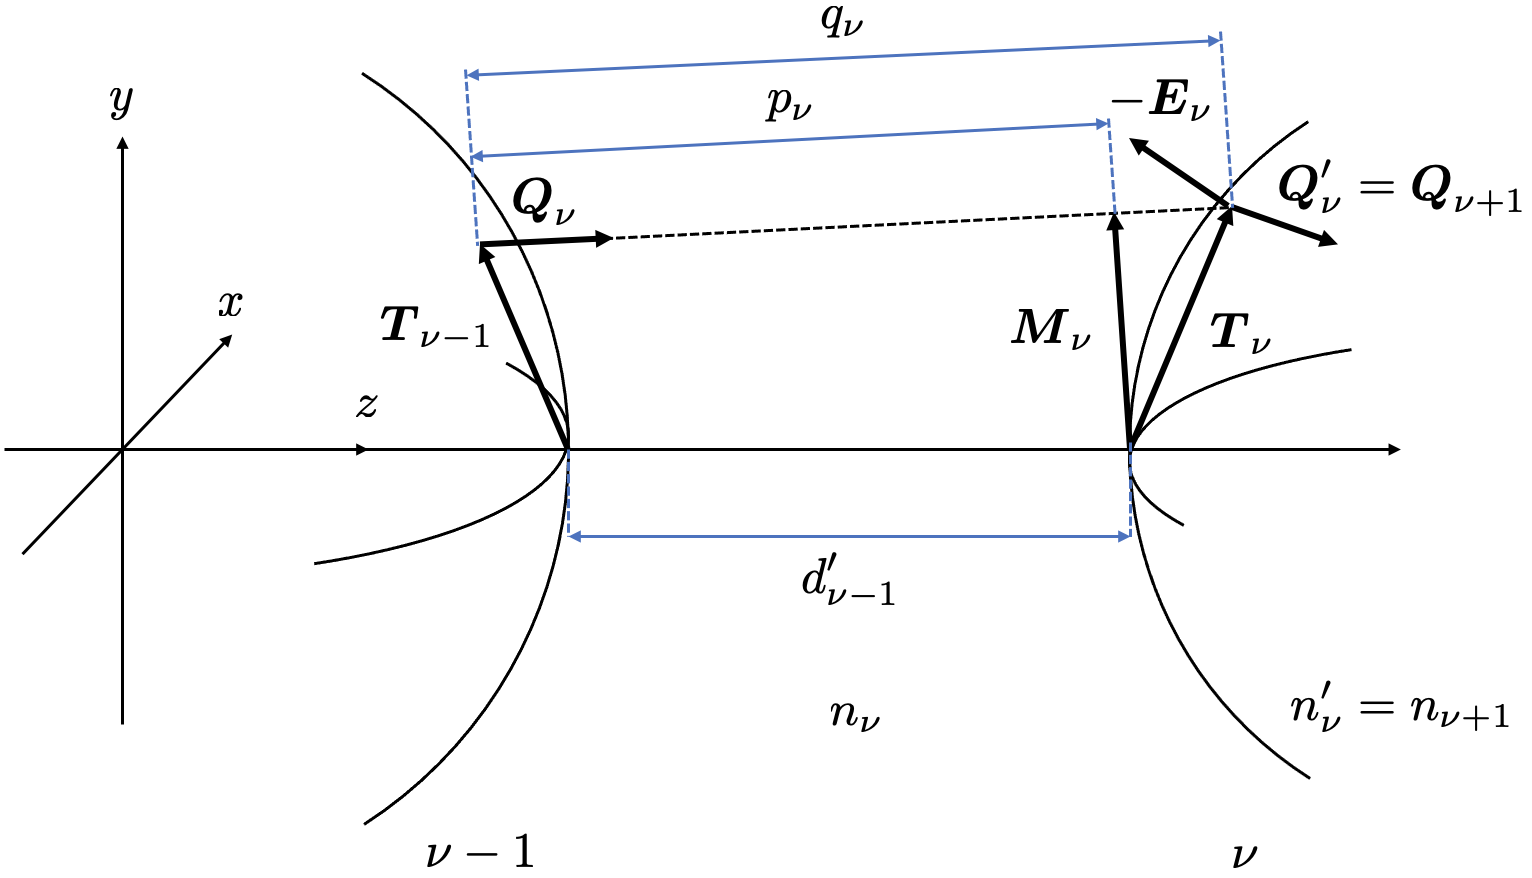
\includegraphics[width=10cm]{ray_tracing_notation.png}
    \caption{光線追跡の notation}
    \label{fig:ray_tracing_notation}
\end{figure}

\begin{table}[b]
    \centering
    \begin{tabular}{l|l}
        記号 & 意味 \\ \hline
        $\vb*{T}_\nu=\qty(x_\nu,\ y_\nu,\ z_\nu)$ & 面 $\nu$ の頂点を始点とした,この面上の光線の通過位置を示すベクトル \\
        $\vb*{Q}_{\nu-1}'=\vb*{Q}_\nu=\qty(q_{\nu x},\ q_{\nu y},\ q_{\nu z})$ & 面$\nu-1$から射出する / 面$\nu$へ入射する光線の方向を示す単位ベクトル\\
        $\vb*{M}_\nu=\qty(m_{\nu x},\ m_{\nu y},\ m_{\nu z})$& 面$\nu$の頂点から$\vb*{Q}_\nu$に下した垂線を表すベクトル \\
        $\vb*{E}_\nu=\qty(e_{\nu x},\ e_{\nu y},\ e_{\nu z})$& 面$\nu$の光線通過点における単位法線ベクトル
    \end{tabular}
    \caption{光線追跡の notation}
    \label{table:ray_tracing_notation}
\end{table}

式\eqref{eq:ray_tracing_1}から式\eqref{eq:ray_tracing_6}は幾何的な関係,式\eqref{eq:ray_tracing_7}はSnellの法則である.既知の値は$\vb*{T}_{\nu-1},\vb*{Q}_\nu, d_{\nu-1}'$であり,ここから式\eqref{eq:ray_tracing_1}から式\eqref{eq:ray_tracing_6}によって$p_\nu, q_\nu, \vb*{T}_\nu,\vb*{M}_\nu,\vb*{E}_\nu$を求めて,その後\eqref{eq:ray_tracing_7}によって$\vb*{Q}_{\nu+1}$を求める
\footnote{
    未知数は14個であり,外積の式が2自由度分しかない(両辺とも$\vb*{E}_\nu$に垂直な面内に閉じる)ことを踏まえると,自由度と式の数は等しくなっている.
}.より詳細には,以下のような順番で解くことができる;
\begin{enumerate}
    \item 式\eqref{eq:ray_tracing_1}に$\vb*{Q}_\nu$との内積をとって
        \begin{equation}
            p_\nu=(d_{\nu-1}'\vb*{e}_z-\vb*{T}_{\nu-1})\cdot\vb*{Q}_\nu
        \end{equation}
    \item さらに式\eqref{eq:ray_tracing_1}から
        \begin{equation}
            \vb*{M}_\nu=\vb*{T}_{\nu-1}+p_\nu\vb*{Q}_\nu-d_{\nu-1}'\vb{e}_x
        \end{equation}
    \item 式\eqref{eq:ray_tracing_2}を式\eqref{eq:ray_tracing_3}に代入し,ノルムをとって二次方程式を解くことで
        \begin{equation}
            q_\nu=p_\nu+\frac{\qty(\dfrac{\abs*{\vb*{M}_\nu}^2}{r_\nu}-2M_{\nu x})}{Q_{\nu x}\qty{1+\qty[1-\dfrac{1}{r_\nu Q_{\nu x}^2}\qty(\dfrac{\abs*{\vb*{M}_\nu}^2}{r_\nu}-2M_{\nu x})]^{1/2}}}
        \end{equation}
    $r_\nu=0$の場合は
        \begin{equation}
            q_\nu=p_\nu
        \end{equation}
    \item さらに式\eqref{eq:ray_tracing_2}から
        \begin{equation}
            \vb*{T}_\nu=\vb*{M}_\nu+(q_\nu-p_\nu)\vb*{Q}_\nu
        \end{equation}
    $r_\nu=0$の場合は
        \begin{equation}
            \vb*{T}_\nu=0
        \end{equation}
    \item そして式\eqref{eq:ray_tracing_3}より
        \begin{equation}
            \vb*{E}_\nu=\vb*{e}_z-\frac{1}{r_\nu}\vb*T_{\nu}
        \end{equation}
    $r_\nu=0$の場合は
        \begin{equation}
            \vb*{E}_\nu=\vb*{e}_z
        \end{equation}
    \item あとは式\eqref{eq:ray_tracing_7}から屈折光線を求めれば良い.$\vb*{E}_\nu$を左から外積として作用させた式
        \begin{equation}
            n_\nu\qty[\vb*{Q}_\nu-\vb*{E}_\nu(\vb*{E}_\nu\cdot\vb*{Q}_\nu)]=n_{\nu+1}\qty[\vb*{Q}_{\nu+1}-\vb*{E}_\nu(\vb*{E}_\nu\cdot\vb*{Q}_{\nu+1})]
        \end{equation}
    から,方向余弦$\xi_\nu, \xi_\nu'$を活用して求められる
    \footnote{
        定義から,$\xi_\nu'\neq \xi_{\nu+1}$であることに注意する.
    }.
        \begin{gather}
            \xi_\nu=\vb*{E}_\nu\cdot\vb*{Q}_\nu\\
            \xi_\nu'=\vb*{E}_\nu\cdot\vb*{Q}_{\nu+1}=\qty[1-\qty(\frac{n_\nu}{n_{\nu+1}})^2\qty(1-\xi_\nu^2)]^{1/2}\\
            n_{\nu+1}\vb*{Q}_{\nu+1}=n_\nu\vb*{Q}_\nu+\qty(n_{\nu}'\xi_\nu'-n_\nu\xi_\nu)\vb*{E}_\nu
            \label{eq:ray_tracing_q}
        \end{gather}
\end{enumerate}

\section{近軸理論}
\label{sec:paraxial_tracing}
光線が光軸に十分近く,光軸との成す角が微小である場合,入射角が微小となるため$\sin i\sim\tan i\sim i$と近似することができる.この場合の結像理論を近軸理論あるいはGauss結像理論と呼ぶ.Gauss結像は,一般の光線の結像位置に対する基準となり,収差の原点となる.よって,レンズ設計は一般の光線の結像位置をどれだけ近軸光線の結像位置に近づけられるかというのが主な仕事になる.

\subsection{光軸付近の光線追跡}
\label{subsec:optical_axis_paraxial_tracing}
まずは1枚の面に関する屈折を考える.記法を図\ref{fig:paraxial_tracing}に示す.
\begin{figure}[b]
    \centering
    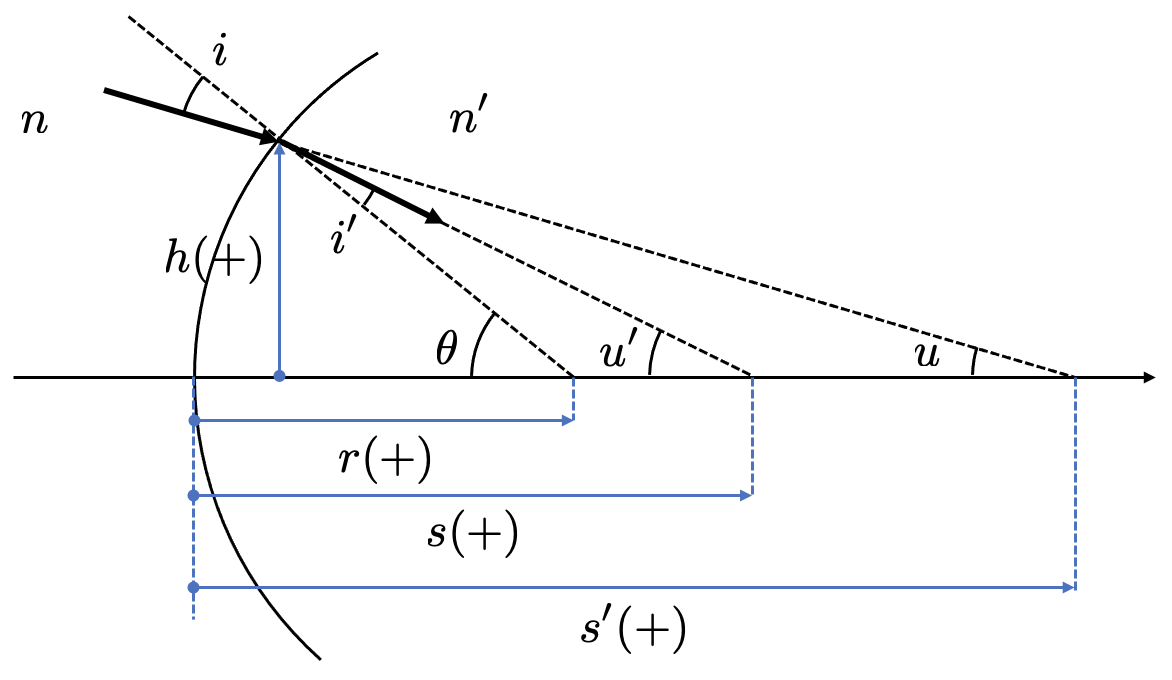
\includegraphics[width=10cm]{paraxial_tracing.png}
    \caption{近軸光線追跡の notation}
    \label{fig:paraxial_tracing}
\end{figure}
幾何的な関係とSnellの法則から
\begin{gather}
    i=\theta-u,\ i'=\theta-u'\\
    \theta=\frac{h}{r},\ u=\frac{h}{s},\ u'=\frac{h}{s'}\\
    n(\theta-u)=n'(\theta-u')
\end{gather}
となり,これらの関係から,Abbeの不変量$Q$の式
\begin{equation}
    Q=n\qty(\frac{1}{r}-\frac{1}{s})=n'\qty(\frac{1}{r}-\frac{1}{s'})
\end{equation}
が導かれ,$h$をかけることで
\begin{gather}
    n'u'=nu+h\varphi\\
    \varphi=\frac{n'-n}{r}
\end{gather}
を導くことができる
\footnote{
    Abbe の不変量と呼ばれているが,屈折面の前後でしか保存しないため,ネーミングとしては微妙である.光学系全体を通して保存しない理由は,式\eqref{eq:ray_tracing_q}の註に書いたように,$\xi_\nu' \neq\xi_{\nu+1}$であることに起因する.
}
.なお,この関係式は\eqref{eq:ray_tracing_q}式の両辺に$-\vb*{e}_y$の内積
\footnote{
    負符号は角度の定義の都合である.
}を作用させることで
\begin{equation}
    n'\sin u'=n\sin u+(n'\xi'-n\xi)\sin\theta
\end{equation}
となり,$\sin u\sim u$ および $\sin\theta=h/r$ と $\xi\sim\xi'\sim 1$ を用いることで得ることもできる.

ここから,複数の面$\nu=1,2,...,k$を通過する場合の近軸追跡式を導くことができる.面$\nu-1,\nu$の面間隔を$d_{\nu-1}'$とする.空気換算量を
\begin{gather}
    \alpha_\nu=n_\nu u_\nu\\
    e_{\nu-1}'=n_\nu d_{\nu-1}'
\end{gather}
と定義することで,近軸光線の追跡公式を以下のように得る;
\begin{gather}
    \alpha_\nu'=\alpha_{\nu+1}=\alpha_\nu +h_\nu\varphi_\nu\\
    h_{\nu+1}=h_\nu-e_\nu'\alpha_\nu'
\end{gather}

\subsection{非点収差の公式}
\label{subsec:astigmatic_paraxial_tracing}
一般の主光線に対して,そのごく近傍の光線に対する光線追跡公式を考える.これは一般には収差論の話題として語られるが,その考え方は近軸理論に近いものであるから,ここでまとめて述べることにする.
%
\begin{figure}
    \centering
    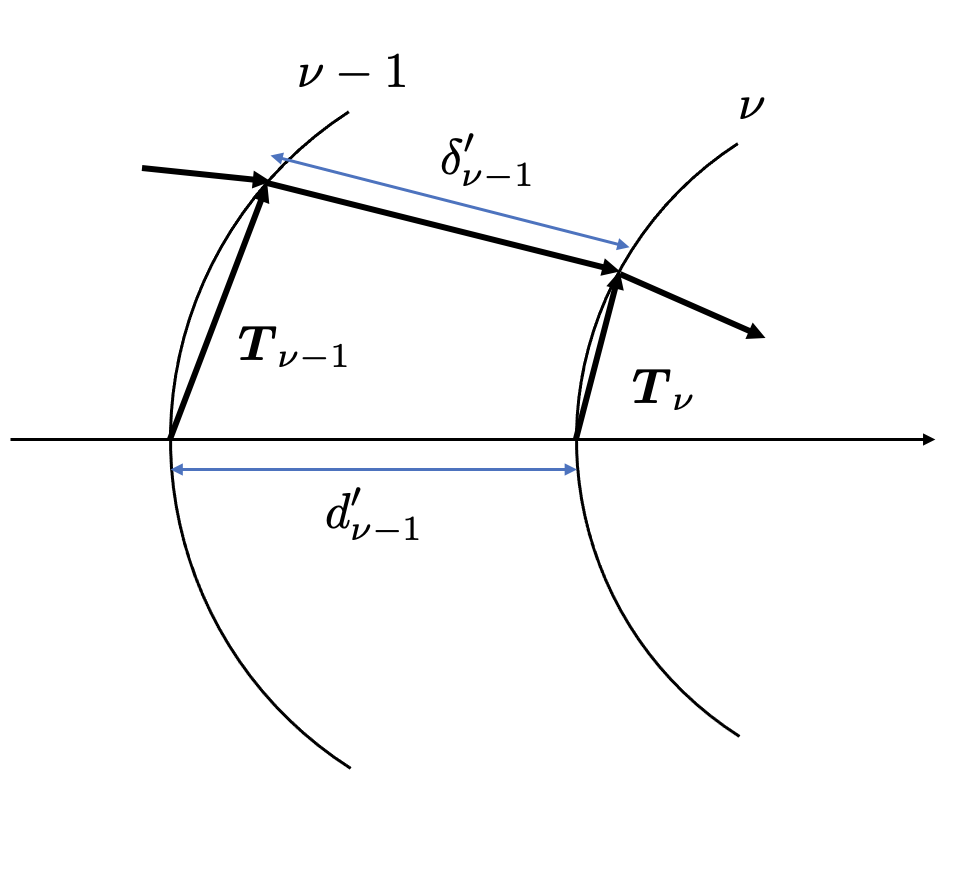
\includegraphics[width=7cm]{surface_distance.png}
    \caption{主光線に沿った面間隔}
    \label{fig:surface_distance}

    \centering
    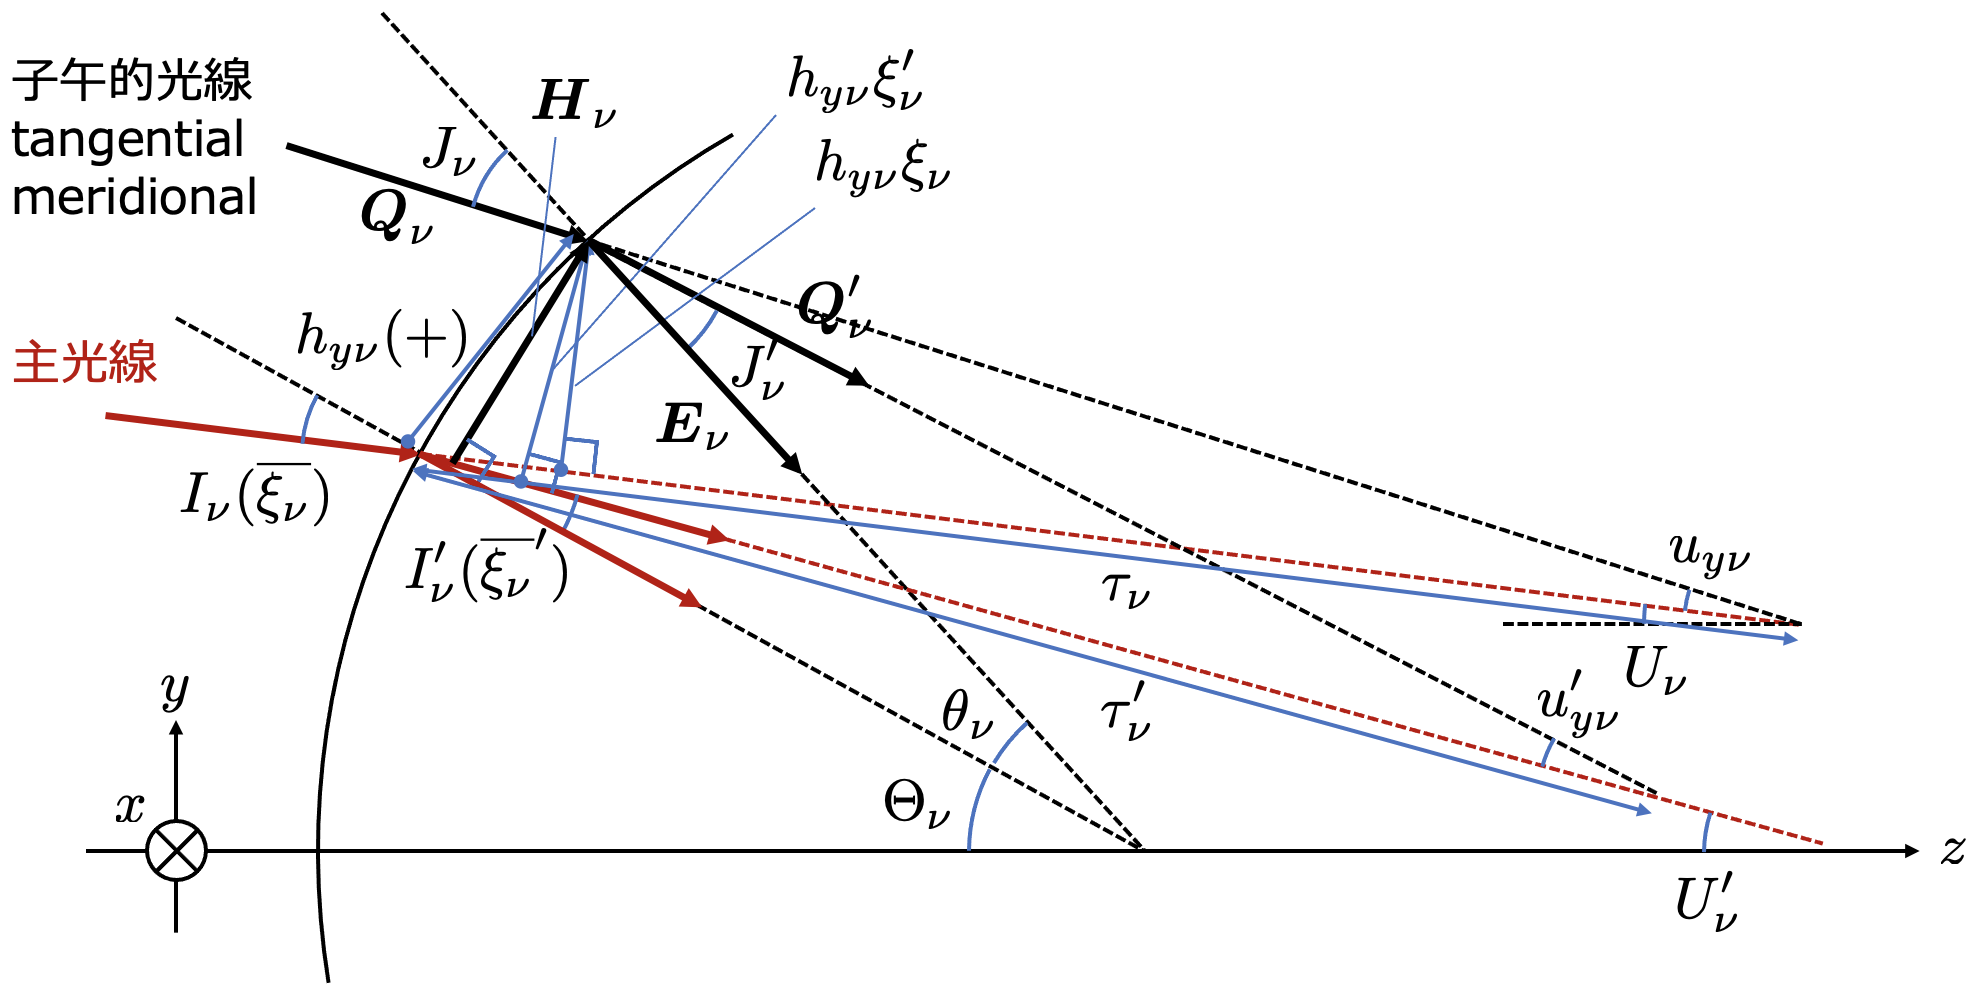
\includegraphics[width=12cm]{tangential_tracing.png}
    \caption{子午的光線の非点追跡}
    \label{fig:tangential_tracing}

    \centering
    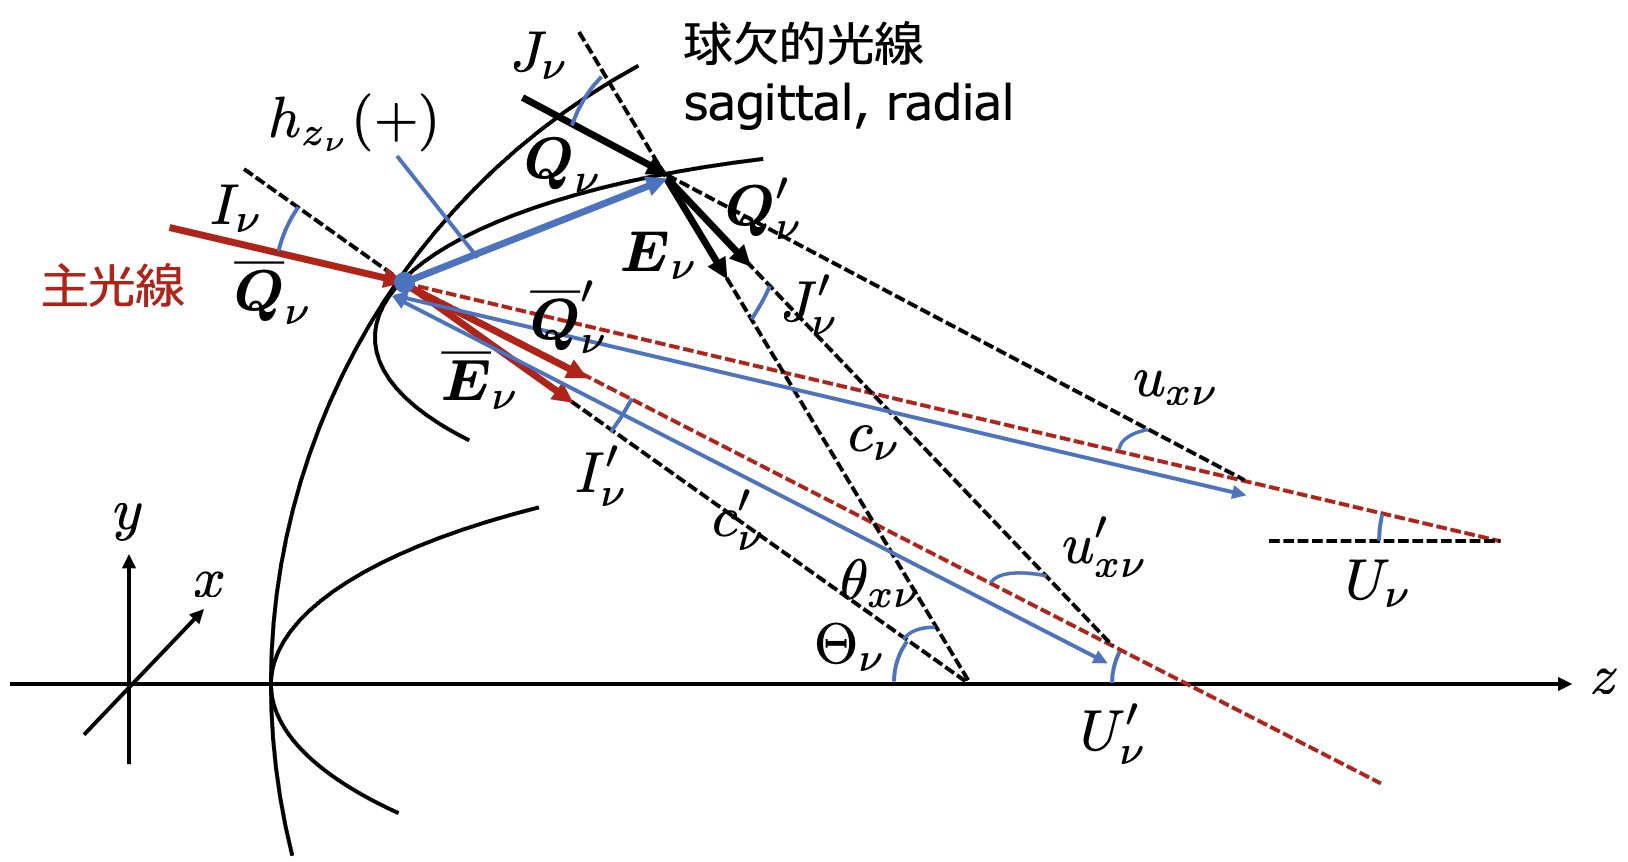
\includegraphics[width=11cm]{sagittal_tracing.png}
    \caption{球欠的光線の非点追跡}
    \label{fig:sagittal_tracing}
\end{figure}

\ref{sec:ray_tracing}節に述べた方法を用いて主光線の追跡ができているとする.このとき図\ref{fig:tangential_tracing}, \ref{fig:sagittal_tracing}
にあるように主光線との成す角がわずかな周辺光線に対して,主光線を光軸だと思って近軸光線追跡を行うのが,非点収差の追跡公式と呼ばれるものである.まず,図\ref{fig:surface_distance}にあるように,主光線に沿った面間隔$\delta$を計算する.
%
\begin{equation}
    \delta_{\nu-1}'=\frac{d_{\nu-1}'+x_\nu-x_{\nu-1}}{q_{\nu x}}
\end{equation}
%
これを用いると,主光線近傍の子午的光線(tangential, meridional)および球欠的光線(sagittal, radial)の追跡式が以下のように求められる;

\paragraph{子午的光線(tangential, meridional)}

\begin{gather}
    n_\nu'u_{y\nu}'\overline{\xi}_{\nu}'=n_\nu u_{y\nu}\overline{\xi}_{\nu}+h_{y\nu}\frac{n_\nu'\overline{\xi}_\nu'-n_\nu\overline{\xi}_\nu}{r_\nu}
    \label{eq:tangential_tracing_1} \\
    u_{y\nu+1}=u_{y\nu}'
    \label{eq:tangential_tracing_2} \\
    h_{y\nu+1}\overline{\xi}_{\nu+1}=h_{y\nu}\overline{\xi}_{\nu}'-\delta_\nu'u_{y\nu}'
    \label{eq:tangential_tracing_3}
\end{gather}

近軸の場合の式と比較すると,tangential面内の通過位置の違いによって発生する傾きを$\xi,\xi'$で適宜修正していることがわかる.また,パワー$\varphi_\nu$は
\begin{equation}
    \frac{n_\nu'-n_\nu}{r_\nu}
    \longrightarrow
    \frac{n_\nu'\overline{\xi}_\nu'-n_\nu\overline{\xi}_\nu}{r_\nu}
\end{equation}
と補正されていることがわかる.

また,
\begin{equation}
    u_{y\nu}=\frac{h_{y\nu}\overline{\xi}_\nu}{\tau_\nu},\ u_{y\nu}'=\frac{h_{y\nu}\overline{\xi}_\nu'}{\tau_\nu'}
\end{equation}
の関係から,収差 $\tau_\nu, \tau_\nu'$ を直接追跡する式も求めることができる;
\begin{equation}
    \frac{n_\nu' {\overline{\xi}_\nu'}^2}{\tau_\nu'}-\frac{n_\nu \overline{\xi}_\nu^2}{\tau_\nu}=\frac{n_\nu'\overline{\xi}_\nu'-n_\nu\overline{\xi}_\nu}{r_\nu}
\end{equation}

\paragraph{球欠的光線(sagittal, radial)}
\begin{gather}
    n_\nu'u_{x\nu}'=n_\nu u_{x\nu}+h_{x\nu}\frac{n_\nu'\overline{\xi}_\nu'-n_\nu\overline{\xi}_\nu}{r_\nu}
    \label{eq:sagittal_tracing_1} \\
    u_{x\nu+1}=u_{x\nu}'
    \label{eq:sagittal_tracing_2} \\
    h_{x\nu+1}=h_{x\nu}-\delta_\nu'u_{x\nu}'
    \label{eq:sagittal_tracing_3}
\end{gather}

近軸の場合の式と比較すると,子午的光線の場合と同様に,主光線のtangential面内の通過位置によって,パワー$\varphi_\nu$が
\begin{equation}
    \frac{n_\nu'-n_\nu}{r_\nu}
    \longrightarrow
    \frac{n_\nu'\overline{\xi}_\nu'-n_\nu\overline{\xi}_\nu}{r_\nu}
\end{equation}
と補正されていることがわかる.

また,
\begin{equation}
    u_{x\nu}=\frac{h_{x\nu}}{c_\nu},\ u_{x\nu}'=\frac{h_{x\nu}}{c_\nu'}
\end{equation}
の関係から,収差 $\tau_\nu, \tau_\nu'$ を直接追跡する式も求めることができる;
\begin{equation}
    \frac{n_\nu'}{c_\nu'}-\frac{n_\nu}{c_\nu}=\frac{n_\nu'\overline{\xi}_\nu'-n_\nu\overline{\xi}_\nu}{r_\nu}
\end{equation}

\paragraph{導出}

子午的光線の場合.まず主光線の追跡は
\begin{gather}
    \overline{\vb*{Q}}_\nu=\mqty(0\\ -\sin U_\nu\\ \cos U_\nu),\ \overline{\vb*{Q}}_\nu'=\mqty(0\\ -\sin U_\nu'\\ \cos U_\nu'),\ \overline{\vb*{E}}_\nu=\mqty(0\\ -\sin \Theta_\nu\\ \cos \Theta_\nu)\\
    \Theta_\nu=I_\nu+U_\nu,\ \Theta_\nu=I_\nu'+U_\nu'
\end{gather}
であり,子午的光線は
\begin{gather}
    \vb*{Q}_\nu=\mqty(0\\ -\sin (U_\nu+u_{y\nu})\\ \cos (U_\nu+u_{y\nu})),\ \vb*{Q}_\nu'=\mqty(0\\ -\sin (U_\nu'+u_{y\nu}')\\ \cos (U_\nu'+u_{y\nu}')),\ \vb*{E}_\nu=\mqty(0\\ -\sin (\Theta_\nu+\theta_\nu)\\ \cos (\Theta_\nu+\theta_\nu))\\
    J_\nu=(\Theta_\nu+\theta_\nu)-(\Theta_\nu-I_\nu+u_{y\nu})\\
    J_\nu'=(\Theta_\nu+\theta_\nu)-(\Theta_\nu-I_\nu'+u_{y\nu}')
\end{gather}
であり
\begin{align}
    &\begin{aligned}
        \xi_\nu
        &=\vb*{Q}_\nu\cdot\vb*{E}_\nu=\cos J_\nu=\cos (I_\nu+\theta_\nu-u_{y\nu})\\
        &=\cos I_\nu \cos (\theta_\nu-u_{y\nu})-\sin I_\nu \sin (\theta_\nu-u_{y\nu})\\
        &\sim \cos I_\nu -\sin I_\nu (\theta_\nu-u_{y\nu})
    \end{aligned}\\
    & \xi_\nu'\sim \cos I_\nu' -\sin I_\nu' (\theta_\nu-u_{y\nu}')
\end{align}
である.式 \eqref{eq:snell} の両辺に
\begin{equation}
    \vb*{H}_\nu=\mqty(0\\ \cos \Theta_\nu\\ \sin \Theta_\nu)
\end{equation}
を作用させる.
\begin{align}
    &\begin{aligned}
        \vb*{H}_\nu\cdot\vb*{Q}_\nu&=\sin(\Theta_\nu-U_\nu-u_{y\nu})=\sin(I_\nu-u_{y\nu})\\
        &=\sin I_\nu\cos u_{y\nu}-\sin u_{y\nu}\cos I_\nu\\
        &\sim \sin I_\nu-\cos I_\nu u_{y\nu}
    \end{aligned}\\
    &\begin{aligned}
        \vb*{H}_\nu\cdot\vb*{E}_\nu&=\sin(\Theta_\nu-\Theta_\nu-\theta_\nu)=\sin(-\theta_\nu)\\
        &\sim -\theta_\nu
    \end{aligned}
\end{align}
より
\begin{equation}
    \begin{aligned}
        &n_\nu(\sin I_\nu-\cos I_\nu u_{y\nu})+n_\nu\theta_\nu[\cos I_\nu -\sin I_\nu (\theta_\nu-u_{y\nu})]\\
        &=n_\nu'(\sin I_\nu'-\cos I_\nu' u_{y\nu}')+n_\nu'\theta_\nu[\cos I_\nu' -\sin I_\nu' (\theta_\nu-u_{y\nu}')]
    \end{aligned}
\end{equation}
ここで,主光線に対する Snell の法則 \eqref{eq:snell}
\begin{equation}
    n_\nu\sin I_\nu=n_\nu'\sin I_\nu'
\end{equation}
と,高次の微小項 $\theta_\nu u_{y_\nu}, \theta_\nu u_{y_\nu}'$を無視すると
\begin{equation}
    -n_\nu u_{y\nu}\cos I_\nu + n_\nu\theta_\nu\cos I_\nu
    =-n_\nu' u_{y\nu}'\cos I_\nu' + n_\nu'\theta_\nu'\cos I_\nu'
\end{equation}
となる.そして
\begin{equation}
    \theta_\nu\sim \frac{h_{y\nu}}{r_\nu}
\end{equation}
の関係から,式\eqref{eq:tangential_tracing_1}が導かれる.式 \eqref{eq:tangential_tracing_2}, \eqref{eq:tangential_tracing_3} については明らかである.

球欠的光線の場合.まず主光線の追跡は
\begin{gather}
    \overline{\vb*{Q}}_\nu=\mqty(0\\ -\sin U_\nu\\ \cos U_\nu),\ 
    \overline{\vb*{Q}}_\nu'=\mqty(0\\ -\sin U_\nu'\\ \cos U_\nu'),\ 
    \overline{\vb*{E}}_\nu=\mqty(0\\ -\sin \Theta_\nu\\ \cos \Theta_\nu)\\
    \Theta_\nu=I_\nu+U_\nu,\ \Theta_\nu=I_\nu'+U_\nu'
\end{gather}
である.子午的光線については,$u_{x\nu}, u_{x\nu}', \theta_x$を$zx$平面に射影した角度がおおよそ
\begin{equation}
    u_{x\nu}\cos U_\nu,\ u_{x\nu}'\cos U_\nu',\ \theta_x\cos\Theta_\nu
\end{equation}
となることを利用して
\begin{align}
    &\begin{aligned}
        \vb*{Q}_\nu&=R_y(-u_{x\nu}\cos U_\nu)\overline{\vb*{Q}}_\nu\\
        &\sim
        \mqty(
            \cos (u_{x\nu}\cos U_\nu) & 0 & -\sin (u_{x\nu}\cos U_\nu)\\
            0 & 1 & 0\\
            \sin (u_{x\nu}\cos U_\nu) & 0 & \cos (u_{x\nu}\cos U_\nu)
        )
        \mqty(
            0\\
            -\sin U_\nu\\
            \cos U_\nu
        )\\
        &\sim \mqty(
            -u_{x\nu}\cos^2 U_\nu\\
            -\sin U_\nu\\
            \cos U_\nu
        )\\
    \end{aligned}\\
    &\vb*{Q}_\nu'\sim
    \mqty(
        -u_{x\nu}'\cos^2 U_\nu'\\
        -\sin U_\nu'\\
        \cos U_\nu'
    )\\
    &\vb*{E}_\nu\sim
    \mqty(
        -\theta_{x\nu}\cos^2 \Theta_\nu\\
        -\sin \Theta_\nu\\
        \cos \Theta_\nu
    )
\end{align}
であり,高次の微小項を無視すれば
\begin{align}
    &\begin{aligned}
        \xi_\nu
        &=\vb*{Q}_\nu\cdot\vb*{E}_\nu\\
        &\sim \sin U_\nu\sin \Theta_\nu + \cos U_\nu \cos \Theta_\nu\\
        &=\cos(\Theta-U_\nu)\\
        &=\overline{\xi}_\nu
    \end{aligned}\\
    & \xi_\nu'\sim \overline{\xi}_\nu'
\end{align}
が得られる.式 \eqref{eq:snell} の両辺に $-\vb*{e}_y$ を内積として作用させると
\begin{align}
    &\begin{aligned}
        \vb*{Q}_\nu\cdot(-\vb*{e}_y)&\sim\sin U_\nu=\sin (I_\nu-\Theta_\nu)\\
        &=\sin I_\nu \cos \Theta_\nu - \cos I_\nu \sin \Theta_\nu
    \end{aligned}\\
    &\vb*{Q}_\nu'\cdot(-\vb*{e}_y)\sim \sin I_\nu' \cos \Theta_\nu - \cos I_\nu' \sin \Theta_\nu\\
    &\vb*{E}_\nu\cdot(-\vb*{e}_y)\sim\sin \Theta_\nu
\end{align}
から
\begin{equation}
    \begin{aligned}
        &n_\nu(\sin I_\nu-\cos I_\nu u_{y\nu})+n_\nu\theta_\nu[\cos I_\nu -\sin I_\nu (\theta_\nu-u_{y\nu})]\\
        &=n_\nu'(\sin I_\nu'-\cos I_\nu' u_{y\nu}')+n_\nu'\theta_\nu[\cos I_\nu' -\sin I_\nu' (\theta_\nu-u_{y\nu}')]
    \end{aligned}
\end{equation}
ここで,主光線に対する Snell の法則 \eqref{eq:snell}
\begin{equation}
    n_\nu\sin I_\nu=n_\nu'\sin I_\nu'
\end{equation}
と,高次の微小項 $\theta_\nu u_{y_\nu}, \theta_\nu u_{y_\nu}'$を無視すると
\begin{equation}
    -n_\nu u_{y\nu}\cos I_\nu + n_\nu\theta_\nu\cos I_\nu
    =-n_\nu' u_{y\nu}'\cos I_\nu' + n_\nu'\theta_\nu'\cos I_\nu'
\end{equation}
となる.そして
\begin{equation}
    \theta_\nu\sim \frac{h_{y\nu}}{r_\nu}
\end{equation}
の関係から,式\eqref{eq:tangential_tracing_1}が導かれる.式 \eqref{eq:tangential_tracing_2}, \eqref{eq:tangential_tracing_3} については明らかである.

\section{収差論}
\label{sec:abberation_theory}

\begin{thebibliography}{99}
\bibitem{ishizaka}石坂,小川,河内,木村,林「量子情報科学入門」共立出版 (2012).

\bibitem{nakahara}中原「理論物理学のための幾何学とトポロジー I」日本評論者 (2018).

\bibitem{yukie1}雪江「代数学1 群論入門」日本評論社 (2010).
\bibitem{yukie2}雪江「代数学2 環と体とガロア理論」日本評論社 (2010).


\bibitem{katsura}桂「代数学$<$2$>$ 環上の加群」東京大学出版会 (2007).
\end{thebibliography}

\end{document}
%%%%%%%%%%%
本文書では,群の準同型定理について述べる.
\begin{screen}
\begin{theo}[群の準同型定理:第一同型定理]\label{第一同型定理}\ \\
$\varphi:G\to H$を群の準同型とする.$\Map{\pi}{G}{G/\Ker{\varphi}}$を自然な準同型とするとき,$\varphi=\psi\circ\pi$となるような準同型$\Map{\psi}{G/\Ker{\varphi}}{H}$がただ一つ存在し,$\psi$は$G/\Ker{\varphi}$から$\Ima{\varphi}$への同型となる.
\begin{center}
\begin{tikzpicture}[auto]
\node (G) at (0, 1.5) {$G$};
\node (H) at (2, 1.5) {$H$};
\node (GKer) at (0, 0) {$G/\Ker{\varphi}$};

\draw[->] (G) to node {$\scriptstyle \varphi$} (H);
\draw[->] (G) to node[swap] {$\scriptstyle \pi$} (GKer);
\draw[->, dashed] (GKer) to node[swap] {$\scriptstyle \psi$} (H);
\end{tikzpicture}
\end{center}
\end{theo}
\end{screen}
\paragraph{証明}
$M=\Ker{\varphi}$とおく.$g\in G$に対し,$\psi(gM)=\varphi(g)$と定義すると,$\Map{\psi}{G/M}{H}$はwell-definedである($\because$ $n\in M$なら,$\varphi(gn)=\varphi(g)\varphi(n)=\varphi(g)1_H=\varphi(g)$となるので,$\psi$は剰余類$gM$の代表元の取り方によらず決まる.).

\begin{shaded}
\begin{defi}[第二加算公理]\ \\
位相空間$(S,\mathfrak{D})$において,たかだか加算の基底$\mathfrak{B}$が存在するとき,$(S,\mathfrak{D})$は第二加算公理を満たすという.
\end{defi}
\end{shaded}

\begin{thebibliography}{9}
\bibitem{雪江}雪江明彦 「代数学1 群論入門」, 日本評論社 (2010).
\end{thebibliography}



\begin{equation}

\end{equation}


\begin{gather}

\end{gather}


\begin{equation}
\begin{pmatrix}

\end{pmatrix}
\end{equation}


\begin{equation}
\begin{split}

\end{split}
\end{equation}